\subsection{Кластеризация слов из электронных писем}

Аналогично кластеризации над письмами Клинтон, была произведена кластеризация над 
электронными письмами $Enron$. Как и ранее, для улучшения качества результатов,
использовалась модель $Word2Vec$, предобученная на датасете постов из $Twitter$, которая затем была <<дообучена>> на корпусе писем $Enron$.

Полученная модель удовлетворяет таким же свойстам, что и ранее: если для слова
взять его векторное представление и найти ближайшие векторные представления других слов, мы
получим близкие по смыслу слова.

Так же была построена интерактивная проекция точек на \textit{2D}-плоскость, однако в данном случае лучших результатов удалось добиться, используя в качестве алгоритма уменьшения размерности $UMAP$, а не \textit{t-SNE}, который использовался для набора Клинтон:

\begin{figure}[H]
\centering
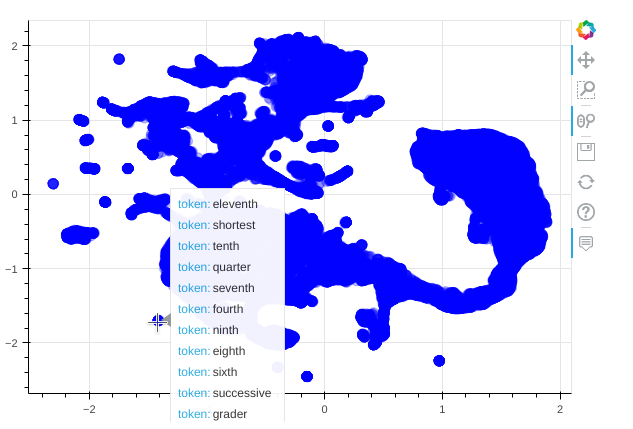
\includegraphics[scale=0.9]{pics/points-2.png}
\caption{Визуализации полученных векторных представлений слов набора $Enron$}
\end{figure}

Как можно заметить, сжатие координат до двумерных прошло успешно, об этом можно судить 
по равмерности распределения полученных точек и выделенному на рисунке скоплению точек ---
этот кластер содержит в себе названия чисел, также есть много других интерпретируемых кластеров.


Для набора $Enron$ также была разработана кластеризация другим алгоритмом:
вместо того, чтобы брать векторные представления слов и их кластеризовать, для каждого письма были усреднены векторные представления всех его слов (по каждой координате), которые далее были кластеризованы с помощью алгоритма $HDBSCAN$ (таким образом количество кластеров определится самостоятельно), предварительно уменьшив размерность векторных представлений
до 5 с помощью $UMAP$. Теперь, для каждого такого кластера можно брать несколько самых близких слов (их векторных представлений). Таким образом получилась кластеризация исходных слов, которая, как оказалось, показывает результаты лучше наивной кластеризации векторных представлений слов. Интуиция, стоящая за этим, может заключаться в том, что смысл той или иной темы определяется всеми предложениями, описывающими эту тему.

Ниже приведены примеры слов, принадлежащие некоторым кластерам (из 1335 полученных):

\begin{table}[H]
\centering
\begin{tabular}{ | l | l | l | }
\hline
Номер кластера & Слова \\ \hline
110 & text, follow, txt, plz, reply, pls, please \\ \hline
3 & hawaii, disneyland, jamaica, alaska, beach, resort,
\\ & skyline, harbor, atlantic, caribbean \\ \hline
54 & angel, queen, princess, prince, savage,
\\ & poetic, explicit, remix, prod, barbie \\ \hline
194 & satisify, vain, endless, definition, quite,
\\ & priceless, compete, successfully, genius \\ \hline
\end{tabular}
\caption{Полученные кластера слов в наборе $Enron$}
\end{table}

Как видно, кластера получились довольно интерпретируемые, например, в кластере 110
некоторые слова написаны по-разному (с опечатками, с сокращением), но модель смогла понять что они по сути означают одно и то же, а в кластере 3 содержатся слова, содержащие названия некоторых географических объектов.
